\documentclass[main.tex]{subfiles}

\begin{document}

\subsection{Rete di moduli per le specie di piante e api nei siti ERAI/ERESP}

La modularità per le specie di piante e api identificate nei siti ERAI e ERESP dell’Emilia-Romagna ha definito il grado di compartimentalizzazione della rete di moduli attraverso le funzioni descritte nel relativo capitolo \ref{Cap. 2.12} e definito i seguenti risultati.
I seguenti dati (Tab. \ref{tab:9}) esprimono il valore di somiglianza associato al valore della modularità per entrambi gli ecosistemi oggetto di studio:

\begin{table}[h!]
    \centering
\begin{tabular}{|1|1|1|}
\hline
~ & Agroecosistema intensivo (AI) & Agroecosistema seminaturale (ES)\\
\hline
Modularità & 0.6771758 & 0.5245437 \\
\hline
\end{tabular}
    \caption{valore della modularità per i siti ERAI es ERESP.}
    \label{tab:9}
\end{table}

Il valore può essere compreso tra 0 e 1. Dove valore 0 significa che la comunità non presenta interazioni tra le parti ed è difficilmente riconducibile a sotto-comunità quali i moduli, mentre il valore 1 indica che la comunità è perfettamente compartimentata e tutte le interazioni sono riconducibili all’interno di un modulo specifico \citep{dormann}.
I grafici sottostanti definiscono i vari network per agroecosistema intensivo (Fig. \ref{fig:moduli ERAI}) e seminaturale (Fig. \ref{fig:moduli ESP}) in base al valore della modularità (verosimiglianza). I quadranti rossi rappresentano i moduli e al loro interno sono indicate le interazioni pesate tra le specie di piante ed il relativo impollinatore, maggiore è la forza dell’interazione e maggiore sarà l’intensità del colore (blu).


\begin{figure}[H]
\centering
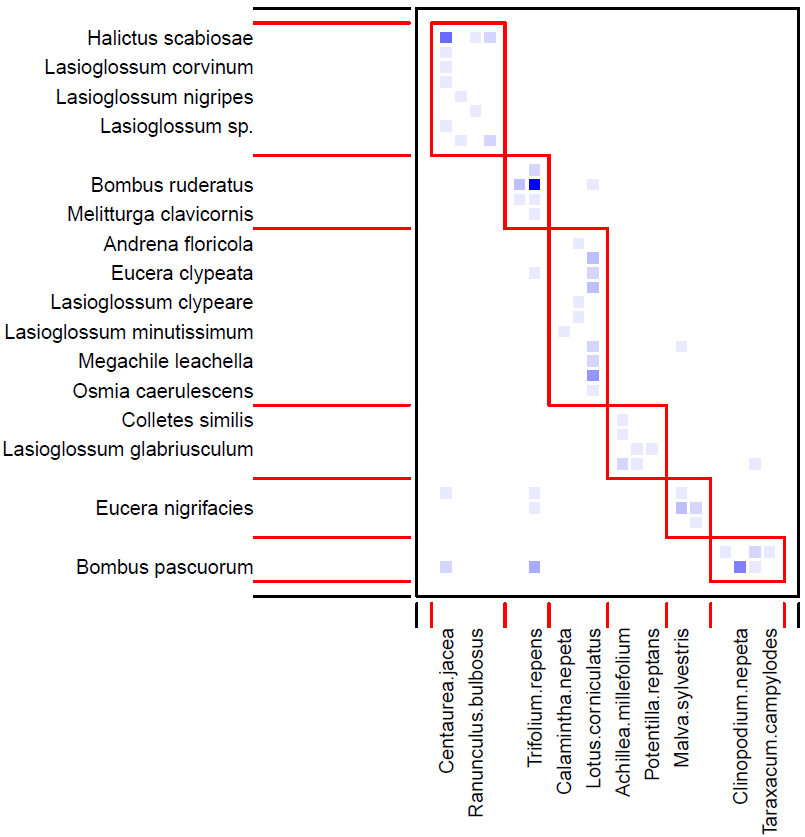
\includegraphics[width=0.6\textwidth]{./Immagini/plotModuleWeb_Network_Api_Piante_AI.png}
\caption{moduli ed interazioni tra piante ed impollinatori del sito ERAI.}
\label{fig:moduli ERAI}
\end{figure}

\begin{figure}[H]
\centering
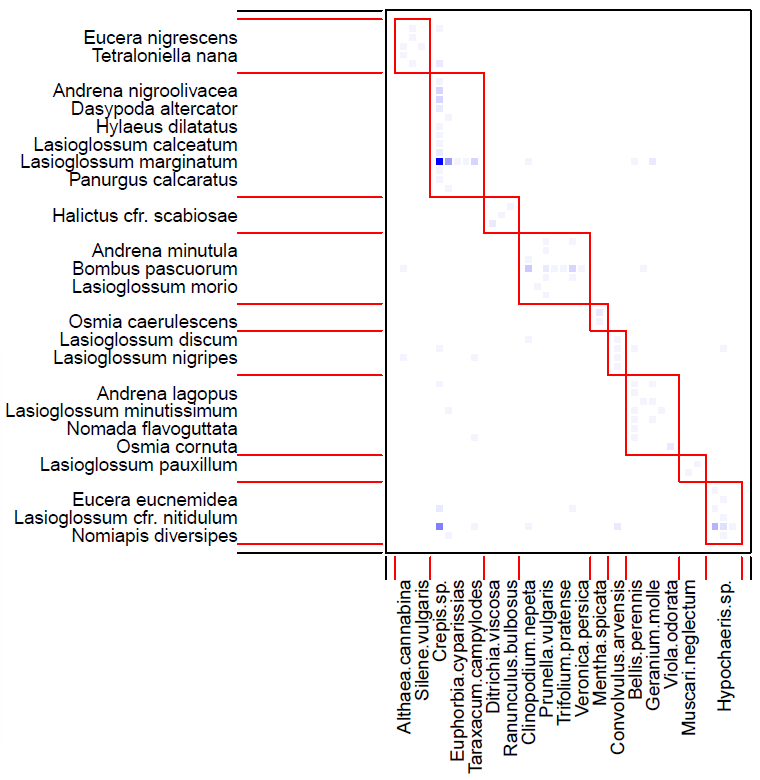
\includegraphics[width=0.6\textwidth]{./Immagini/plotModuleWeb_Network_Api_Piante_ESP.png}
\caption{moduli ed interazioni tra piante ed impollinatori del sito ESP.}
\label{fig:moduli ESP}
\end{figure}

Le interazioni pianta/impollinatore che si trovano all’interno dello stesso modulo costituiscono legami tra le parti più solidi rispetto alle interazioni tra elementi di moduli differenti.

\clearpage

\end{document}





